%%%%%%%%%%%%  Generated using docx2latex.com  %%%%%%%%%%%%%%

%%%%%%%%%%%%  v2.0.0-beta  %%%%%%%%%%%%%%

\documentclass[12pt]{article}
\usepackage{amsmath}
\usepackage{latexsym}
\usepackage{amsfonts}
\usepackage[normalem]{ulem}
\usepackage{soul}
\usepackage{array}
\usepackage{amssymb}
\usepackage{extarrows}
\usepackage{graphicx}
\usepackage[backend=biber,
style=numeric,
sorting=none,
isbn=false,
doi=false,
url=false,
]{biblatex}\addbibresource{bibliography.bib}

\usepackage{subfig}
\usepackage{wrapfig}
\usepackage{wasysym}
\usepackage{enumitem}
\usepackage{adjustbox}
\usepackage{ragged2e}
\usepackage[svgnames,table]{xcolor}
\usepackage{tikz}
\usepackage{longtable}
\usepackage{changepage}
\usepackage{setspace}
\usepackage{hhline}
\usepackage{multicol}
\usepackage{tabto}
\usepackage{float}
\usepackage{multirow}
\usepackage{makecell}
\usepackage{fancyhdr}
\usepackage[toc,page]{appendix}
\usepackage[hidelinks]{hyperref}
\usetikzlibrary{shapes.symbols,shapes.geometric,shadows,arrows.meta}
\tikzset{>={Latex[width=1.5mm,length=2mm]}}
\usepackage{flowchart}\usepackage[paperheight=11.0in,paperwidth=8.5in,left=1.0in,right=1.0in,top=1.0in,bottom=1.0in,headheight=1in]{geometry}
\usepackage[utf8]{inputenc}
\usepackage[T1]{fontenc}
\TabPositions{0.5in,1.0in,1.5in,2.0in,2.5in,3.0in,3.5in,4.0in,4.5in,5.0in,5.5in,6.0in,}

\urlstyle{same}

\renewcommand{\_}{\kern-1.5pt\textunderscore\kern-1.5pt}

 %%%%%%%%%%%%  Set Depths for Sections  %%%%%%%%%%%%%%

% 1) Section
% 1.1) SubSection
% 1.1.1) SubSubSection
% 1.1.1.1) Paragraph
% 1.1.1.1.1) Subparagraph


\setcounter{tocdepth}{5}
\setcounter{secnumdepth}{5}


 %%%%%%%%%%%%  Set Depths for Nested Lists created by \begin{enumerate}  %%%%%%%%%%%%%%


\setlistdepth{9}
\renewlist{enumerate}{enumerate}{9}
		\setlist[enumerate,1]{label=\arabic*)}
		\setlist[enumerate,2]{label=\alph*)}
		\setlist[enumerate,3]{label=(\roman*)}
		\setlist[enumerate,4]{label=(\arabic*)}
		\setlist[enumerate,5]{label=(\Alph*)}
		\setlist[enumerate,6]{label=(\Roman*)}
		\setlist[enumerate,7]{label=\arabic*}
		\setlist[enumerate,8]{label=\alph*}
		\setlist[enumerate,9]{label=\roman*}

\renewlist{itemize}{itemize}{9}
		\setlist[itemize]{label=$\cdot$}
		\setlist[itemize,1]{label=\textbullet}
		\setlist[itemize,2]{label=$\circ$}
		\setlist[itemize,3]{label=$\ast$}
		\setlist[itemize,4]{label=$\dagger$}
		\setlist[itemize,5]{label=$\triangleright$}
		\setlist[itemize,6]{label=$\bigstar$}
		\setlist[itemize,7]{label=$\blacklozenge$}
		\setlist[itemize,8]{label=$\prime$}



 %%%%%%%%%%%%  Header here  %%%%%%%%%%%%%%


\pagestyle{fancy}
\fancyhf{}
\cfoot{ \setlength{\parskip}{0.0pt}
}
\renewcommand{\headrulewidth}{0pt}
\setlength{\topsep}{0pt}\setlength{\parskip}{9.96pt}
\setlength{\parindent}{0pt}

 %%%%%%%%%%%%  This sets linespacing (verticle gap between Lines) Default=1 %%%%%%%%%%%%%%


\renewcommand{\arraystretch}{1.3}


%%%%%%%%%%%%%%%%%%%% Document code starts here %%%%%%%%%%%%%%%%%%%%



\begin{document}
\begin{Center}
\textbf{Understanding plasmon dispersion in nearly-free-electron metals: the relevance of exact constraints for novel exchange-correlation kernels within time-dependent density functional theory}
\end{Center}\par

\begin{Center}
\textbf{Niraj K. Nepal\textsuperscript{1},\textsuperscript{ }Santosh Adhikari\textsuperscript{1}, Bimal Neupane\textsuperscript{1}, Shiqi Ruan\textsuperscript{1}, Santosh Neupane\textsuperscript{1 }}
\end{Center}\par

\begin{Center}
\textbf{and Adrienn Ruzsinszky\textsuperscript{1}}
\end{Center}\par

\setlength{\parskip}{0.0pt}
\begin{Center}
\textsuperscript{1}\textit{ Department of Physics, Temple University, Philadelphia, PA, 19122}
\end{Center}\par


\vspace{\baselineskip}
\setlength{\parskip}{9.96pt}
\setlength{\parskip}{0.0pt}
\begin{Center}
\textbf{Abstract}
\end{Center}\par


\vspace{\baselineskip}
\setlength{\parskip}{9.96pt}
\setlength{\parskip}{0.0pt}
\begin{justify}
 Small-wavevector excitations in Coulomb-interacting systems can be decomposed into the high-energy collective longitudinal plasmon and the low-energy single-electron excitations. At the critical wavevector and corresponding frequency where the plasmon branch merges with the single-electron excitation region, the collective energy of the plasmon dissipates into single electron-hole excitations. The jellium model provides a reasonable description of the energy-loss spectrum of metals close to the free-electron limit in the long-wavelength limit. The random phase approximation (RPA) is exact in the high-density limit but can capture the plasmonic dispersion reasonably even for densities with rs >1. RPA results in a wrong infinite plasmon lifetime for a wavevector smaller than the critical one where the plasmon dispersion curve runs into particle-hole excitations. The impact of the exchange-correlation kernels can be significant and kernels modify the plasmon dispersion curve. There is however a large difference in the construction and performance of the kernels investigated earlier. Our current work introduces recent model exchange-only and exchange-correlation kernels and discusses the relevance of some exact constraints in the construction of the kernel. This work completes our understanding about the plasmon dispersion in realistic metals, where anomalous behavior was observed with RPA. 
\end{justify}\par


\vspace{\baselineskip}
\setlength{\parskip}{9.96pt}
\setlength{\parskip}{0.0pt}
\begin{justify}
\textbf{Introduction}
\end{justify}\par


\vspace{\baselineskip}
\setlength{\parskip}{9.96pt}
\setlength{\parskip}{0.0pt}
\begin{justify}
Due to its computational feasibility and relatively high accuracy, approximate Kohn-Sham density-functional theory (KS-DFT) simulations are the basis of present-day first-principles computational materials science \textsuperscript{1}. Light-particle interactions require beyond semilocal KS-DFT treatment \textsuperscript{2}. Experimental applications in photovoltaics and surface photochemistry heavily rely on understanding and guiding electron-light interaction. A relevant example of light-matter interaction is scattering when an electron is scattered from a crystal resulting in energy loss of the electron. Experimentally the electron loss spectrum can be realized by electron energy loss spectroscopy or by inelastic scattering \textsuperscript{3, 4}. 
\end{justify}\par

\begin{justify}
Excited states can be accurately characterized by expensive Green’s function techniques. By virtue of the Runge-Gross theorem \textsuperscript{5} DFT can be extended to time-dependent processes. Time-dependent density-functional theory (TDDFT) is becoming an attractive alternative to many-body perturbation theory and can offer, in principle, an unbiased and independent framework complementary to experimental observations, enabling the interpretation of specific experimental observations and predictions of new materials with targeted properties.
\end{justify}\par

\begin{justify}
Plasmon excitations are collective oscillations of electrons in the absence of an external electric field, that incorporate Coulomb interaction between electrons \textsuperscript{6}. Due to the electron-electron interactions, plasmon excitations establish a high barrier when testing \textit{ab initio} theories. When the external perturbation is weak, linear response TDDFT \textsuperscript{7}\ is a useful tool to describe optical excitation energies. In TDDFT the electron loss or photoabsorption cross-section is quantified by the imaginary part of $ \chi $ , the spatially nonlocal and dynamic density-density response function. The poles of the interacting density-density response function contain information about the optical excitation energies. The same density-density response function can deliver further information about the plasmon decay for a range of wavevectors.  
\end{justify}\par

\begin{justify}
Plasmon dispersion in nearly-free-electron alkali metals has attracted a great interest among experimentalists and theorists. The deviation in the volume plasmon dispersion of the low-density alkali metals such as Rb and Cs has triggered a debate about the origin of the anomaly observed by most theoretical approximations within TDDFT and Fermi liquid theories \textsuperscript{8}. A strong failure of approximations based on TDDFT is the lack of a damping mechanism which results in an infinite lifetime of plasmons for a region of wavevectors smaller than the critical wavevector that separates plasmonic and particle-hole excitations \textsuperscript{8, 9}. The negative plasmon dispersion in low-density alkali metals, and in general the damping mechanism can be attributed to correlation effects or band structure \textsuperscript{10,-13}. There are pros and contras both explanations in the literature \textsuperscript{12, 13}. In heavier alkali metals such as Cs electron transition to the near-Fermi-level \textit{3d} bands can occur \textsuperscript{10, 11}. The transition energy of these electrons is comparable to the plasmon energy, potentially causing a negative dispersion. Additional corrections to the interacting response function or dielectric function can originate in a weak lattice potential and core polarization effects \textsuperscript{8}. 
\end{justify}\par

\begin{justify}
The random phase approximation (RPA) is a Green’s function-based method that is often used to obtain the ground-state correlation energy of bulk and two-dimensional materials \textsuperscript{14}. Although RPA relies on the linear response TDDFT framework, its excitation energies are inaccurate because of the missing short-range exchange-correlation effects \textsuperscript{15}. The exact exchange-correlation kernel that would provide these effects is a functional derivative of the exchange-correlation potential. RPA is often interpreted within DFT to have roots in the adiabatic connection fluctuation dissipation theorem \textsuperscript{16}. The bare RPA without a band structure does not yield a negative dispersion in heavy alkali metals \textsuperscript{10}. Some investigations of the role of correlation in the plasmon dispersion discuss kernels, but most tests consider the exchange-correlation effects at the level of adiabatic local density functional approximation (ALDA) only. The work of Tatarczyk et al. \textsuperscript{17} steps beyond this limitation to some extent by considering some more model kernels based either on the uniform electron gas paradigm or on other constraints.
\end{justify}\par

\begin{justify}
In our current work we aim to fill the gap in analyzing the plasmon dispersion with recent exchange-correlation kernels, beyond the early ones developed in the 90’s. Our work aims to go beyond a simple analysis of exchange-correlation effects with kernels. The major goal here is to give an \textit{a priori }numerical analysis why kernels by themselves (without the band-structure effects) can not predict negative dispersion in low density alkali metals. In this work we rely on the jellium model. We demonstrate that even without the band structure effects the exact constraints can lead to kernels that correctly predict a positive plasmon dispersion in jellium.
\end{justify}\par


\vspace{\baselineskip}
\setlength{\parskip}{9.96pt}
\setlength{\parskip}{0.0pt}
\begin{justify}
\textbf{Methodology: Exchange-correlation kernels within linear response TDDFT}
\end{justify}\par


\vspace{\baselineskip}
\setlength{\parskip}{9.96pt}
\setlength{\parskip}{0.0pt}
\begin{justify}
Nonempirical construction of density functionals has allowed widespread and successful applications of these approximations for the ground state \textsuperscript{18}. Various exact constraints such as the uniform electron gas limit, Lieb-Oxford bound or the one-electron limit are known for the ground state \textsuperscript{19}.\ Some of these exact constraints are also natural starting point when constructing exchange-correlation kernels within linear response TDDFT for excited states.  According to linear response theory the interacting and noninteracting density-density response functions are coupled by the Dyson equation:
\end{justify}\par


\vspace{\baselineskip}
\setlength{\parskip}{9.96pt}
\setlength{\parskip}{0.0pt}
\begin{Center}
\ \ \ \ \ \ \ \ \ \ \ \ \ \ \ \   \(  \chi _{ \lambda } \left( q, \omega  \right) =  \chi _{0} \left( q, \omega  \right) + \chi _{0} \left( q, \omega  \right)  \left(  \lambda v_{c} \left( q \right) +f_{xc}^{ \lambda } \left( q, \omega  \right)  \right)  \chi _{ \lambda } \left( q, \omega  \right)  \) \ \ \ \ \ \ \ \ \ \ \ \ \ \ \ \ \ \ \ \ \ \ \ \ \ \ \ \ \ \ \ \ \ \ \ \ \ \  (1)
\end{Center}\par


\vspace{\baselineskip}
\setlength{\parskip}{9.96pt}

\vspace{\baselineskip}
\setlength{\parskip}{0.0pt}
\setlength{\parskip}{9.96pt}
\setlength{\parskip}{0.0pt}
\begin{justify}
 \(  \chi _{ \lambda } \left( q, \omega  \right)  \) \ and   \(  \chi _{0} \left( q, \omega  \right)  \)  are the interacting and noninteracting response functions, respectively,  \( v_{c} \left( q \right) =\frac{4 \pi }{q^{2}} \)  and  \( f_{xc}^{ \lambda } \left( q, \omega  \right)  \)  are the Coulomb and exchange-correlation kernels. $ \lambda $  is the coupling constant that represents the adiabatic connection between a noninteracting Kohn-Sham and the interacting real system response. When Eq. (1) is applied to the uniform electron gas,  \(  \chi _{0} \left( q, \omega  \right)  \)  becomes the Lindhard function with complex frequencies \textsuperscript{20}, a basic component of our current research. 
\end{justify}\par

\begin{justify}
In the adiabatic approximation, the exact kernel is a second functional derivative of the ground state exchange-correlation energy. In practice the exact kernel is unknown but can be modeled by satisfying exact physical constraints. Kernels are related to the $``$local field factors$"$  as  \( G \left( q, \omega  \right) = \frac{f_{xc}^{ \lambda } \left( q, \omega  \right) }{-v_{c} \left( q \right) }. \) 
\end{justify}\par

\begin{justify}
Many real systems have densities close to the paradigm uniform electron gas as in alkali metals. The uniform electron gas is therefore a well-justified system for an exact constraint. All exchange-correlation kernels in this work model the uniform electron gas with known limiting behavior at q \(  \rightarrow 0 \)  and q \(  \rightarrow \infty. \)  The simplest approximation is known as the adiabatic local density approximation (ALDA) kernel \textsuperscript{21}:
\end{justify}\par


\vspace{\baselineskip}
\setlength{\parskip}{9.96pt}
\setlength{\parskip}{0.0pt}
\begin{Center}
\ \ \ \ \ \ \ \ \ \ \ \ \ \ \ \ \ \ \ \ \ \ \ \ \ \ \ \ \ \ \ \ \ \ \   \( f_{xc}^{ALDA} \left( q \rightarrow 0,  \omega =0 \right) =-\frac{4 \pi A}{k_{F}^{2}} \) \ \ \ \ \ \ \ \ \ \ \ \ \ \ \ \ \ \ \ \ \ \ \ \ \ \ \ \ \ \ \ \ \ \ \ \ \ \ \ \ \ \ \ \ \ \ \ \ \ \ \ \  (2)
\end{Center}\par


\vspace{\baselineskip}
\setlength{\parskip}{9.96pt}
\setlength{\parskip}{0.0pt}
\begin{justify}
with  \( A=\frac{1}{4}-\frac{k_{F}^{2}}{4 \pi }\frac{d^{2} \left( n \varepsilon _{c} \right) }{dn^{2}} \) ,\  where  \( k_{F}= \left( 3 \pi ^{2}n \right) ^{1/3} \)  is the Fermi wavevector and  \(  \varepsilon _{c} \)  the correlation energy per particle of the uniform electron gas.  \( A=\frac{1}{4} \)  belongs only to the exchange-only ALDA, while the density-dependent term in  \( A \)  gives the correlation beyond the high-density limit.
\end{justify}\par

\begin{justify}
The real-space representation of ALDA is a the delta function which indicates the spatial locality of this kernel. ALDA gives reasonable accuracy for low-frequency, long-wavelength excitations, but is not the right choice for a correction to RPA \textsuperscript{21}. The ALDA kernel was applied to the ground state correlation energy of the uniform electron gas but makes an error of $ \sim $ 0.5 eV \textsuperscript{22}. This error is the same in magnitude but of opposite sign to the error that RPA makes for the same system.
\end{justify}\par

\begin{justify}
The ALDA kernel can be made nonlocal, by applying a cutoff that makes the exchange-correlation kernel cancel the Hartree kernel for q > 2k\textsubscript{F}. The cutoff is introduced by the renormalized ALDA (rALDA) expression \textsuperscript{23}
\end{justify}\par


\vspace{\baselineskip}
\setlength{\parskip}{9.96pt}
\setlength{\parskip}{0.0pt}
\begin{Center}
\ \ \ \ \ \ \ \ \ \ \ \ \ \ \ \ \ \ \ \ \ \ \ \ \ \ \ \ \   \( f_{xc}^{rALDA} \left( n,q \right) =- \left[  \theta  \left( k_{cut}-q \right) \frac{4 \pi }{k_{cut}^{2}}+ \theta  \left( q-k_{cut} \right) \frac{4 \pi }{q^{2}} \right] , \) \ \ \ \ \ \ \ \ \ \ \ \ \ \ \ \ \ \ \ \ \ \ \ \ \ \ \ \ \ \ \ \ \ \ \ \ \ \ \ \ \ \ \ \ \ \ \ \ \  (3)
\end{Center}\par


\vspace{\baselineskip}
\setlength{\parskip}{9.96pt}
\setlength{\parskip}{0.0pt}
\begin{justify}
\ with the cutoff wavevector   \( k_{cut}=\frac{k_{F}}{\sqrt{A}}. \) \ \ By construction the rALDAxc kernel keeps the correct  q \(  \rightarrow 0 \)  limit of ALDA, but corrects the wrong q \(  \rightarrow \infty \) \  behavior of ALDAxc.\  
\end{justify}\par

\begin{justify}
For inhomogeneous systems, more ingredients like the density gradient or the kinetic energy density give more flexibility for kernels, as for ground state density functional approximations. The kinetic energy density is one of the ingredients of the nonlocal energy optimized (NEO) exchange-only kernel \textsuperscript{24}.
\end{justify}\par

\begin{justify}
The NEO kernel improves the ground state correlation energy beyond RPA and structural properties. The NEO kernel is designed to satisfy further physical constraints beyond both ALDA or rALDA, and has the form
\end{justify}\par


\vspace{\baselineskip}
\setlength{\parskip}{9.96pt}
\setlength{\parskip}{0.0pt}
\begin{Center}
\ \ \ \ \ \ \ \ \ \ \ \ \ \ \ \ \ \ \ \ \ \ \ \ \ \ \ \ \ \ \ \ \ \ \ \ \ \ \ \ \ \ \ \ \ \   \( f_{x}^{NEO}=\frac{4 \pi }{q^{2}} \left[ 1-e^{- \beta q^{2}/k_{F}^{2}} \right] , \) \ \ \ \ \ \ \ \ \ \ \ \ \ \ \ \ \ \ \ \ \ \ \ \ \ \ \ \ \ \ \ \ \ \ \ \ \ \ \ \ \ \ \ \ \ \ \ \ \ \ \ \ \ \ \ \ \ \ \  (4)
\end{Center}\par


\vspace{\baselineskip}
\setlength{\parskip}{9.96pt}
\setlength{\parskip}{0.0pt}
\begin{justify}
where  \(  \beta =\frac{1}{4\widetilde{c} \left( 1-z^{2} \right) }. \) \  The one-electron limit is satisfied by the ingredient  \( z=\frac{ \tau^{w}}{ \tau}, \)  where  \(  \tau^{w} \)  is the one-electron kinetic energy density \textsuperscript{25} and  \(  \tau \)  the positive kinetic energy density constructed from the Kohn-Sham orbitals. In the uniform electron gas,  \( z \)  is zero, when q \(  \rightarrow 0, \) \ \  the NEO kernel is properly independent of q for the uniform electron gas. The parameter  \( \widetilde{c} \)  has a key relevance to the current work. In the construction of NEO  \( \widetilde{c} \)  is designed to give a correction to the RPA correlation energy in the high-density limit. In other words, the standard  \( \widetilde{c}=0.264 \) \ parameter in NEO provides a unique fit to the exact second-order correlation energy for the spin-unpolarized electron gas.  The $``$second-order exchange$"$  contribution to the second-order correlation energy of the uniform gas is the correction to direct RPA from wavefunction anti-symmetry that survives in the high-density limit. It can be evaluated from explicit expressions given by von Barth and Hedin for RPA \textsuperscript{26} and by Langreth and Perdew \textsuperscript{15}\  beyond RPA.
\end{justify}\par

\begin{justify}
 \(  \beta  \)  can be chosen to satisfy another constraint relevant to the long-wavelength ( \( q \rightarrow 0 \right)  \)  limit. This choice is also made in the CP07 dynamic exchange-correlation kernel constructed by Constantin and Pitarke \textsuperscript{27}. The compressibility sum rule, \textsuperscript{28} as
\end{justify}\par

\begin{Center}
\ \ \ \ \ \ \ \ \ \ \ \ \ \ \ \ \ \ \ \ \ \ \ \ \ \ \ \ \ \ \ \ \ \ \   \( f_{xc}= \left( n;q \rightarrow 0,  \omega =0 \right) =\frac{d^{2}}{dn^{2}} \left[ n \varepsilon _{xc} \left( n \right)  \right] , \) \ \ \ \ \ \ \ \ \ \ \ \ \ \ \ \ \ \ \ \ \ \ \ \ \ \ \ \ \ \ \ \ \ \ \ \ \ \ \ \ \ \ \ \ \ \ \ \ \ \ \ \  (5)
\end{Center}\par


\vspace{\baselineskip}
\setlength{\parskip}{9.96pt}
\setlength{\parskip}{0.0pt}
\begin{justify}
 is an important requirement for frequency-dependent exchange-correlation kernels. Satisfying the compressibility sum rule  \(  \beta  \)  becomes
\end{justify}\par


\vspace{\baselineskip}
\setlength{\parskip}{9.96pt}
\begin{Center}
\ \ \ \ \ \ \ \ \ \ \ \ \ \ \ \ \ \ \ \ \ \ \ \ \ \ \ \ \ \ \ \ \ \ \ \ \ \ \ \ \ \ \   \(  \beta =-\frac{k_{F}}{4 \pi }\frac{d^{2}}{dn^{2}} \left[ n \varepsilon _{xc} \left( n \right)  \right] =A, \) \ \ \ \ \ \ \ \ \ \ \ \ \ \ \ \ \ \ \ \ \ \ \ \ \ \ \ \ \ \ \ \ \ \ \ \ \ \ \ \ \ \ \ \ \ \ \ \ \ \ \ \ \ \ \ \ \ \ \ \ \ \ \ \ \ \ \ \ \ \ \ \ \ \ \ \ \  (6)
\end{Center}\par

\setlength{\parskip}{0.0pt}
\begin{justify}
or\   \( \widetilde{c}=0.5 \)  in the high-density limit.
\end{justify}\par

\begin{justify}
Thus the energy optimization of  \( \widetilde{c}=0.264 \)  in the high-density limit is different from the value  \( \widetilde{c}=0.5 \) \  that yields the correct small- \( q \)  kernel in the high-density limit. In the next section we will extensively discuss the impact of these physical constraints on the plasmon dispersion and provide a novel insight about the role of correlation effects.
\end{justify}\par


\vspace{\baselineskip}
\setlength{\parskip}{9.96pt}

\vspace{\baselineskip}
\setlength{\parskip}{0.0pt}
\setlength{\parskip}{9.96pt}
\setlength{\parskip}{0.0pt}
\begin{justify}
\textbf{Plasmon dispersion with spatially nonlocal exchange-correlation kernels in nearly-free-electron metals}
\end{justify}\par


\vspace{\baselineskip}
\setlength{\parskip}{9.96pt}

\vspace{\baselineskip}
\setlength{\parskip}{0.0pt}
\setlength{\parskip}{9.96pt}
\setlength{\parskip}{0.0pt}
\begin{justify}
The alkali metals Na and K are nearly-free-electron (NFE) systems and therefore ideal models for the uniform electron gas. Correlation effects in alkali metals can be strong enough especially for low electron densities to impact electronic excitations. The high-resolution electron energy loss experiments (EELS) experiments indicate that the plasmon dispersion in heavy alkali metals such as Rb and Cs becomes negative in momentum-transfer q \textsuperscript{8}. Collective plasmon excitations have triggered a long-standing debate about the origin of the negative dispersion found in these heavy alkali metals. Theoretical predictions from the late 80’s in polycrystalline metals showed negative dispersion for Cs beyond RPA when the band structure was included \textsuperscript{29}.\ \ RPA exhibits a positive plasmon dispersion within the jellium model, but was found to lower the dispersion when periodic boundary conditions were present.  Weak lattice potential core polarization effects may be incuded in the plasmon frequencies, even within RPA. Since all the above experiments and calculations were performed for periodic crystals, it is difficult to decouple correlation and band structure effects in the decay of the plasmon excitations.
\end{justify}\par

\begin{justify}
Further calculations by Ku and Eguiluz in K crystal \textsuperscript{11}\ indicate the relevance of band structure versus correlation and demonstrate that the exchange-correlation effects beyond RPA at the ALDA level have only a minor role in the decay of plasmons. A similar observation was made by Quong and Eguiluz  \textsuperscript{30} for Na crystal.
\end{justify}\par

\begin{justify}
Although\ crystal\ periodicity is important when modeling realistic conditions, the jellium model can offer an important way to separate the impact of many-body correlations and band structure. Within our work we want to provide an additional theoretical and numerical insight only about the many-body correlation effects and explain why in general no beyond-RPA approximation for jellium can predict the correct plasmon decay and lifetime for Cs. The justification of our results is based merely on exact physical constraints imposed on the construction of beyond-RPA approximations.  By using the jellium model for alkali metals, we can build upon the conclusion that ALDA gives a minor improvement beyond RPA. With the possession of nonlocal exchange-correlation kernels developed since  the later 90’s we can make further conclusions about how these recent approximations compare to ALDA and RPA in terms of correlation effects.
\end{justify}\par

\begin{justify}
TDDFT\ has become a promising and affordable tool to assess the optical properties of solids. Most of the tests on optical properties still rely on the ALDA approximation. The shortcomings of ALDA become obvious for ground state correlation energies and for excitations of wide-frequency range in inhomogeneous systems. Relying on the observations by Refs  \textsuperscript{11, 30} we can keep the ALDA as our reference method when we compare the plasmon dispersion obtained from other exchange-correlation kernels to ALDA.
\end{justify}\par

\begin{justify}
We can make two groups regarding our approximations assessed. The first group includes exchange-only and exchange-correlation kernels based on the ALDA approximations. ALDAx and ALDAxc are both local kernels but differ in correlation contribution. rALDAx and rALDAxc are nonlocal. The second group consists of NEO exchange-only kernels \textsuperscript{24} with the c parameter constructed by satisfying different physical constraints. By default, the NEO kernel yields the exact high-density limit compared to RPA obtained as
\end{justify}\par


\vspace{\baselineskip}
\setlength{\parskip}{9.96pt}
\setlength{\parskip}{0.0pt}
\begin{Center}
\ \ \ \ \ \ \ \ \ \ \ \ \ \ \ \ \ \ \ \ \ \ \ \ \ \ \ \ \   \( e_{c}^{2X}=\frac{3}{8 \pi ^{3}} \int _{0}^{\infty}dQQ^{2}\widetilde{G}_{x} \left( Q \right)  \int _{0}^{\infty}dWQ^{2} \left\{ 2 \beta  \right} ^{2}, \) \ \ \ \ \ \ \ \ \ \ \ \ \ \ \ \ \ \ \ \ \ \ \ \ \ \ \ \ \ \ \ \ \ \ \ \ \ \ \ \ \ \ \ \ \ \ \ \ \ \ \ \ \ \ \ \ \ \ \ \ \ \ \ \ \ \ \ \  (7)
\end{Center}\par


\vspace{\baselineskip}
\setlength{\parskip}{9.96pt}
\setlength{\parskip}{0.0pt}
\begin{justify}
where  \( \widetilde{G}_{x} \left( Q \right)  \)  refers to the kernel according to the correspondence of kernels and local-field factors.  \( Q=\frac{k}{2k_{F}} \)  is a dimensionless wavevector, and  \( W=\frac{ \Omega }{2k_{F}^{2}} \) \ is a dimensionless frequency to obtain the explicit expression for the second-order exchange energy   \( e_{c}^{2X} \)  by Langreth and Perdew \textsuperscript{15} beyond RPA using the RPA correlation energy for the uniform electron gas given by von Barth and Hedin. The c parameter that corresponds to the second-order correlation energy was found to be 0.264. 
\end{justify}\par

\begin{justify}
The exchange-only NEO kernel for the uniform electron gas at the long-wavelength limit is
\end{justify}\par


\vspace{\baselineskip}
\setlength{\parskip}{9.96pt}
\setlength{\parskip}{0.0pt}
\begin{Center}
\ \ \ \ \ \ \ \ \ \ \ \ \ \ \ \ \   \( f_{x} \left( n;q \rightarrow 0 \right) =\frac{4 \pi }{2k_{F}^{2}}\frac{1}{4\widetilde{c}}. \) \ \ \ \ \ \ \ \ \ \ \ \ \ \ \ \ \ \ \ \ \ \ \ \ \ \ \ \ \ \ \ \ \ \ \ \ \ \ \ \ \ \ \ \ \ \ \ \ \ \ \ \ \ \ \ \ \ \ \ \ \ \ \ \  (8)
\end{Center}\par


\vspace{\baselineskip}
\setlength{\parskip}{9.96pt}
\setlength{\parskip}{0.0pt}
\begin{justify}
Alternatively,\ in the long-wavelength limit we can use the compressibility sum rule formulated as   \( \frac{d^{2}}{dn^{2}} \left[ n \varepsilon _{xc} \left( n \right)  \right]  \)  to determine $``$ \( \widetilde{c} \) $"$ . Then the c parameter of NEO can be estimated from the compressibility sum rule of the ALDAxc expression. This fitting delivers us a different  \( \widetilde{c} \cong  \) 0.44\ at metallic densities.  While formally the NEO approximation remains an exchange-only kernel, this kind of fitting to an exact physical condition with an exchange-correlation approach brings the correlation effects relevant for metallic densities in our NEO kernel \textsuperscript{27}.
\end{justify}\par

\begin{justify}
Clearly $``$c$"$  controls the correlation or screening within the NEO approximation starting from  \( c \rightarrow \infty \) \ in RPA. The impact of $``$c$"$  as a screening parameter on ground state correlation energies was established by Bates et al in 2016.  Changing $``$c$"$  from its default 0.264 value was shown to yield different correlation energy in the uniform electron gas at r\textsubscript{s}=4. 
\end{justify}\par

\begin{justify}
The exchange-only NEO kernel can be explicitly turn into an exchange-correlation approach by replacing $``$ \( \widetilde{c} \) $"$  by an electron-density-dependent parameter. This approach was tested for jellium slab correlation energies for different than high-densities, and resulted in improved integrated correlation energy \textsuperscript{31}. For a given density, the density dependence can make $``$ \( \widetilde{c} \) $"$  significantly smaller than its default value. In our analysis we investigate the effect of a low $``$ \( \widetilde{c} \) $"$  parameter on the plasmon dispersion of various NFE metals. For testing purposes we choose  \( \widetilde{c}=0.0037. \)  Notice that this choice of  \( \widetilde{c} \)  represents an unphysically low density according to Eq. (13) of ref. \textsuperscript{31}. 
\end{justify}\par

\begin{justify}
At\ first we discuss the plasmon dispersion up to the wavevector region where plasmons decay into single particle excitations. We consider all the exchange-correlation kernels described above.  
\end{justify}\par

\begin{justify}
Within the static approximation for the kernel  \( f_{xc} \left( q \right) , \)  the plasmon frequency  \(  \omega _{p} \left( q \right)  \)  is found by solving the equation  \(  \epsilon  \left( q, \omega  \right) =1- \left( v_{c} \left( q \right) +f_{xc} \left( q \right)  \right)  \chi _{0} \left( q \right) =0, \)  for  \(  \lambda =1,  \) \textsuperscript{17} and the solutions are undamped outside the particle-hole contiunuum, i.e., for  \( q<q_{c} \)  where  \( \frac{ \omega _{p} \left( q \right) }{ \varepsilon _{F}}=2 \left( \frac{q_{c}}{k_{F}} \right) + \left( \frac{q_{c}}{k_{F}} \right) ^{2}. \)  For the r\textsubscript{s }values considered here,  \( q_{c}/k_{F} \ll k_{cut}/k_{F} \approx 2, \)  where  \( k_{cut} \) \  is the cutoff wavevector for a kernel.
\end{justify}\par

\begin{justify}
Al is a metal with rather high density, and RPA becomes relatively exact in the high-density limit \textsuperscript{30}. The small wavevector behavior is demonstrated by the correct plasmon energy known from an EELS experiment \textsuperscript{32}. All ALDA and rALDA kernels return the correct long-wavelength limit of RPA. The c \(  \cong  \) 0.44\  NEO exchange kernel keeps the correct long-wavelength of RPA. Since the compressibility sum rule delivers direct information about the long-wavelength limit, among all the approximations NEO c \(  \cong  \) 0.44 has a direct impact on the curvature of the dispersion. The fitting against this exact constraint designates that the plasmon dispersion must start out as horizontal at small wavevectors. NEO c \(  \cong  \) 0.44 exemplifies the best behavior at small wavevectors that any static kernel can demonstrate.
\end{justify}\par

\begin{justify}
Comparing the ALDA and rALDA kernels at the left panel it is apparent that the nonlocal feature of the rALDA so much relevant in the ground state correlation energy does not change the plasmon dispersion and all ALDA and rALDA approximations yield the same dispersion curve. The NEO  \( \widetilde{c} \) =0.264 and  \( \widetilde{c} \) =0.44 methods basically agree, while the NEO c=0.0037 is completely unphysical with low plasmon frequencies as an indication of the lack of exact constraints.
\end{justify}\par


\vspace{\baselineskip}
\setlength{\parskip}{9.96pt}

\vspace{\baselineskip}
\setlength{\parskip}{0.0pt}
\setlength{\parskip}{9.96pt}

\vspace{\baselineskip}
\setlength{\parskip}{0.0pt}
\setlength{\parskip}{9.96pt}


%%%%%%%%%%%%%%%%%%%% Figure/Image No: 1 starts here %%%%%%%%%%%%%%%%%%%%


\begin{figure}[H]	\begin{subfigure}		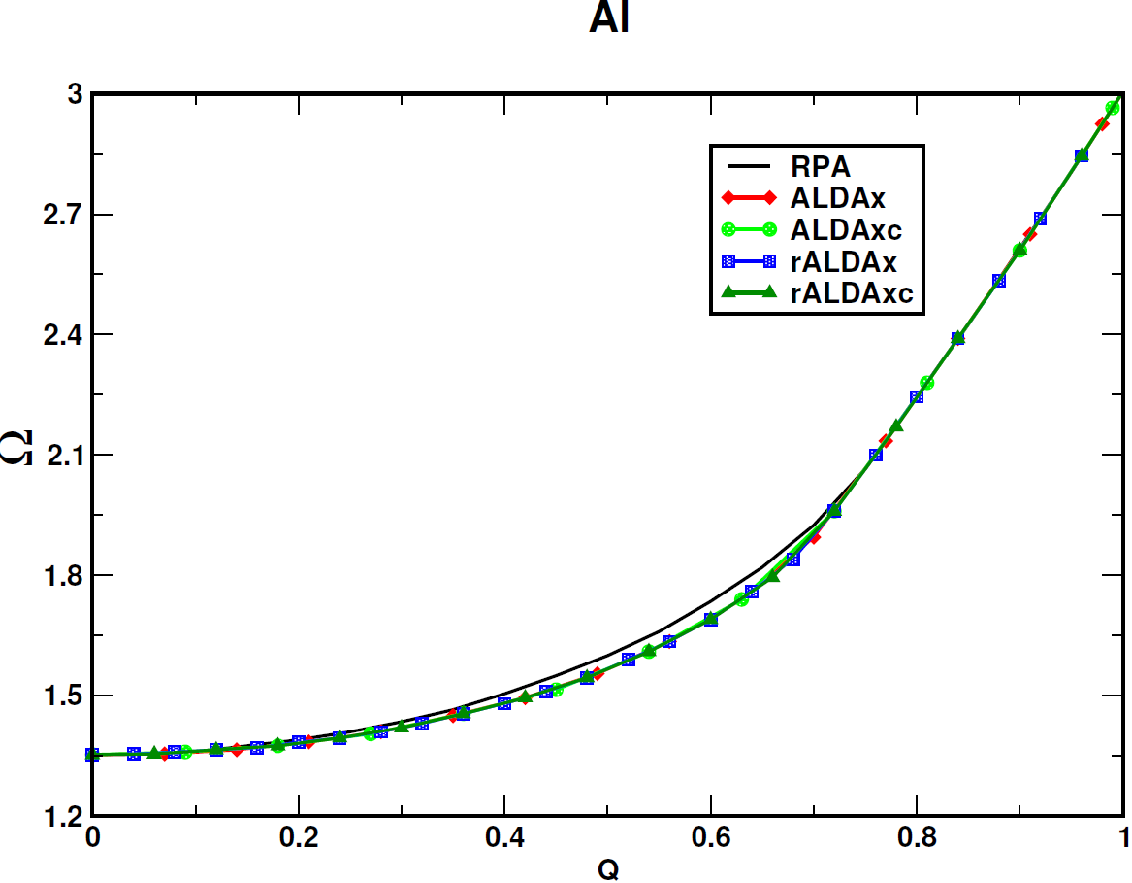
\includegraphics[width=0.45\textwidth]{./media/image2.png}
	\end{subfigure}
~	\begin{subfigure}		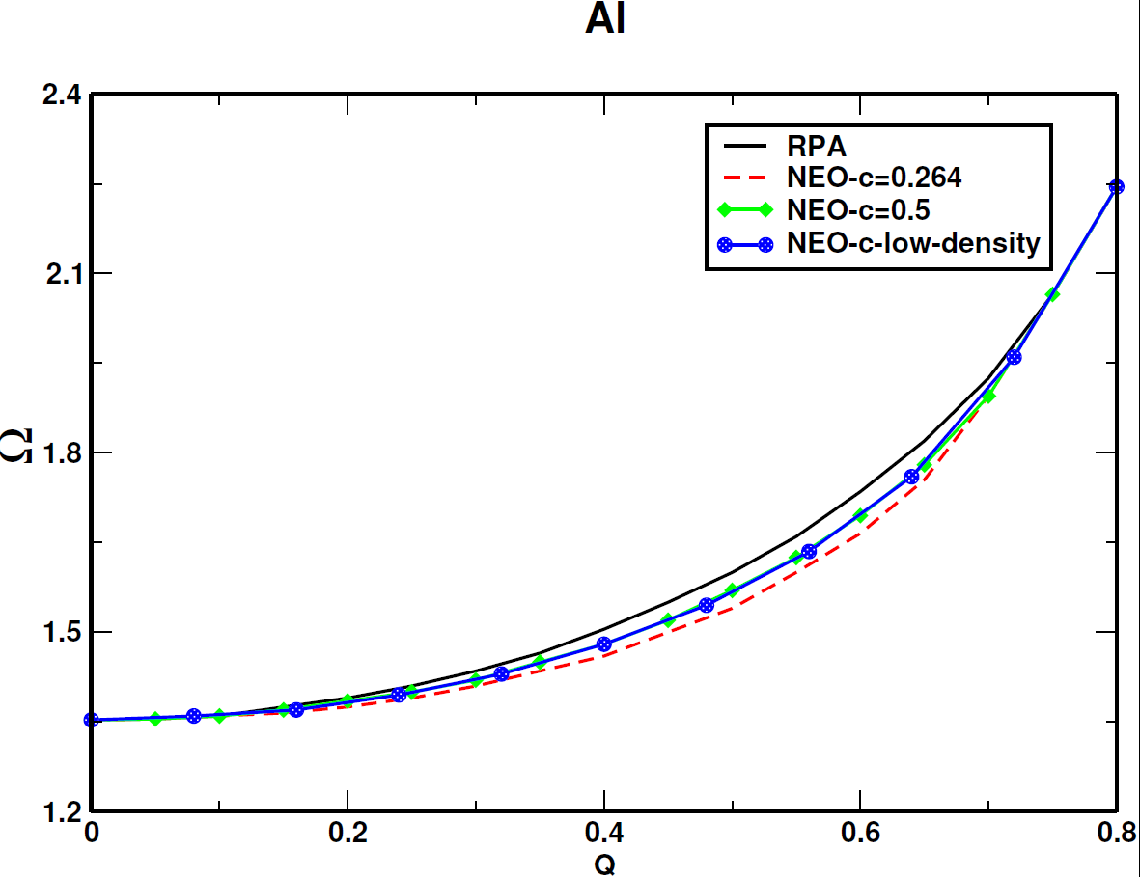
\includegraphics[width=0.45\textwidth]{./media/image13.png}
	\end{subfigure}
~
\end{figure}


%%%%%%%%%%%%%%%%%%%% Figure/Image No: 1 Ends here %%%%%%%%%%%%%%%%%%%%

\setlength{\parskip}{0.0pt}
\par


\vspace{\baselineskip}
\setlength{\parskip}{9.96pt}

\vspace{\baselineskip}
\setlength{\parskip}{0.0pt}
\setlength{\parskip}{9.96pt}
\setlength{\parskip}{0.0pt}
\begin{justify}
\textbf{Fig 1. }The plasmon dispersion for Al up to the critical wavevector. The left panel shows the dispersion obtained with RPA and beyond-RPA with ALDAx, ALDAxc, rALDAx and rALDAxc approximations. The right panel shows the dispersion from RPA and the three NEO approximations with the  \( \widetilde{c} \)  parameters corresponding to different choices.
\end{justify}\par


\vspace{\baselineskip}
\setlength{\parskip}{9.96pt}

\vspace{\baselineskip}
\setlength{\parskip}{0.0pt}
\setlength{\parskip}{9.96pt}
\setlength{\parskip}{0.0pt}
\begin{justify}
For Na with r\textsubscript{s}=3.93, all ALDA and rALDA dispersion curves barely differ in the left panel. Like in Al there is no improvement from the nonlocal kernels. According to the right figure the NEO  \( \widetilde{c}=0.264 \)  and NEO  \( \widetilde{c}=0.44 \)  kernels differ more than they do in Al for a range of $ \sim $ 0.5 for dimensionless wavevector Q. NEO  \( \widetilde{c}=0.0037 \)  leads to unphysically low plasmon frequencies. 
\end{justify}\par


\vspace{\baselineskip}
\setlength{\parskip}{9.96pt}

\vspace{\baselineskip}
\setlength{\parskip}{0.0pt}
\setlength{\parskip}{9.96pt}


%%%%%%%%%%%%%%%%%%%% Figure/Image No: 2 starts here %%%%%%%%%%%%%%%%%%%%


\begin{figure}[H]	\begin{subfigure}		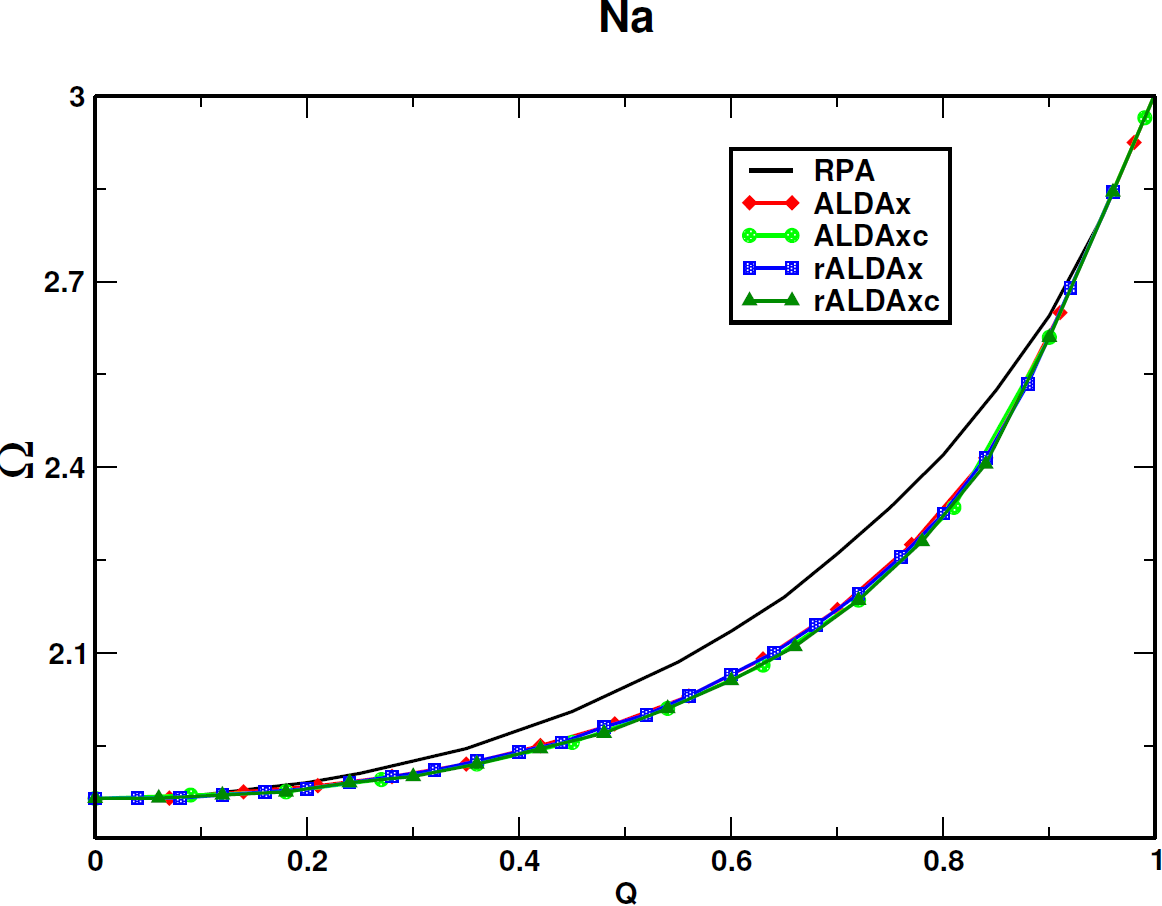
\includegraphics[width=0.45\textwidth]{./media/image5.png}
	\end{subfigure}
~	\begin{subfigure}		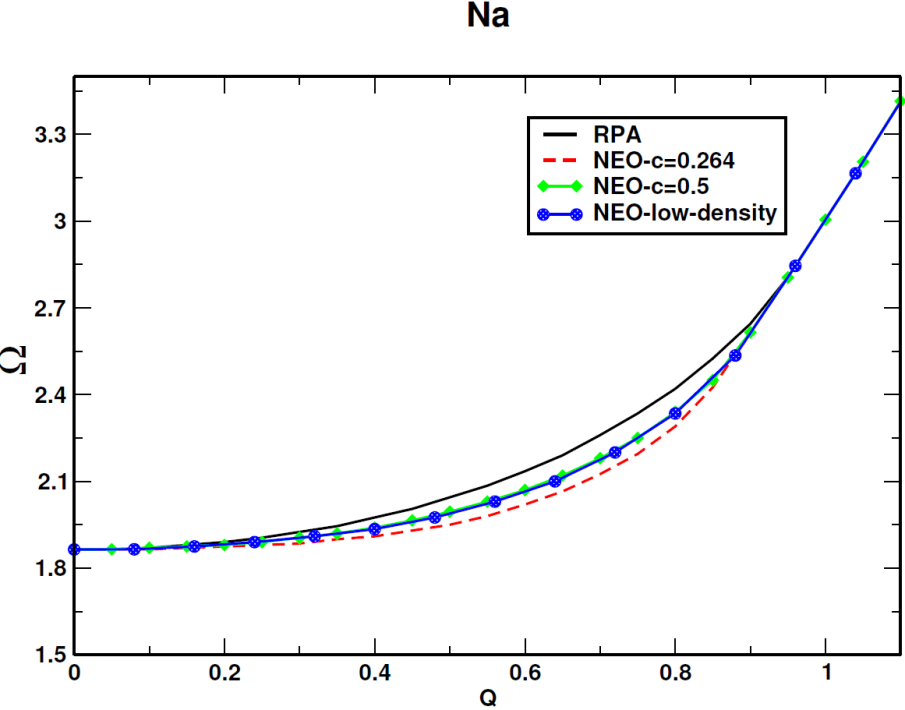
\includegraphics[width=0.45\textwidth]{./media/image6.png}
	\end{subfigure}
~
\end{figure}


%%%%%%%%%%%%%%%%%%%% Figure/Image No: 2 Ends here %%%%%%%%%%%%%%%%%%%%

\setlength{\parskip}{0.0pt}
\par


\vspace{\baselineskip}
\setlength{\parskip}{9.96pt}
\setlength{\parskip}{0.0pt}
\begin{justify}
\textbf{Fig 2. }The plasmon dispersion for Na up to the critical wavevector. The left panel shows the dispersion obtained with RPA and beyond-RPA with ALDAx, ALDAxc, rALDAx and rALDAxc approximations. The right panel shows the dispersion from RPA and the three NEO approximations with the  \( \widetilde{c} \)  parameters corresponding to different choices.
\end{justify}\par


\vspace{\baselineskip}
\setlength{\parskip}{9.96pt}
\setlength{\parskip}{0.0pt}
\begin{justify}
Cs is the alkali metal with the lowest density \textsuperscript{33}. This characteristic manifests itself in the plasmon dispersion when comparing the approximations in the left and right panels of Fig. 3. Being correct at small  \( q, \) \ the ALDAxc and rALDAxc  are more suitable for lower densities in Cs, however, the nonlocality versus locality in rALDAxc and ALDAxc does not affect the dispersion. Comparing the NEO approximations NEO  \( \widetilde{c}=0.264 \)  results in more correction beyond-RPA than it does in the previous two metals. Furthermore NEO  \( \widetilde{c}=0.264 \)  yields more correction in the plasmon frequencies than any of the ALDA and rALDA kernels. The exact constraint-based NEO  \( \widetilde{c}=0.43 \)  behaves more like ALDAx or ALDAxc. NEO  \( \widetilde{c}=0.0037 \)  considerably lowers the plasmon dispersion against the other approximations. At the first glance this could be the desired behavior for the low-density Cs.
\end{justify}\par


\vspace{\baselineskip}
\setlength{\parskip}{9.96pt}

\vspace{\baselineskip}
\setlength{\parskip}{0.0pt}
\setlength{\parskip}{9.96pt}


%%%%%%%%%%%%%%%%%%%% Figure/Image No: 3 starts here %%%%%%%%%%%%%%%%%%%%


\begin{figure}[H]	\begin{subfigure}		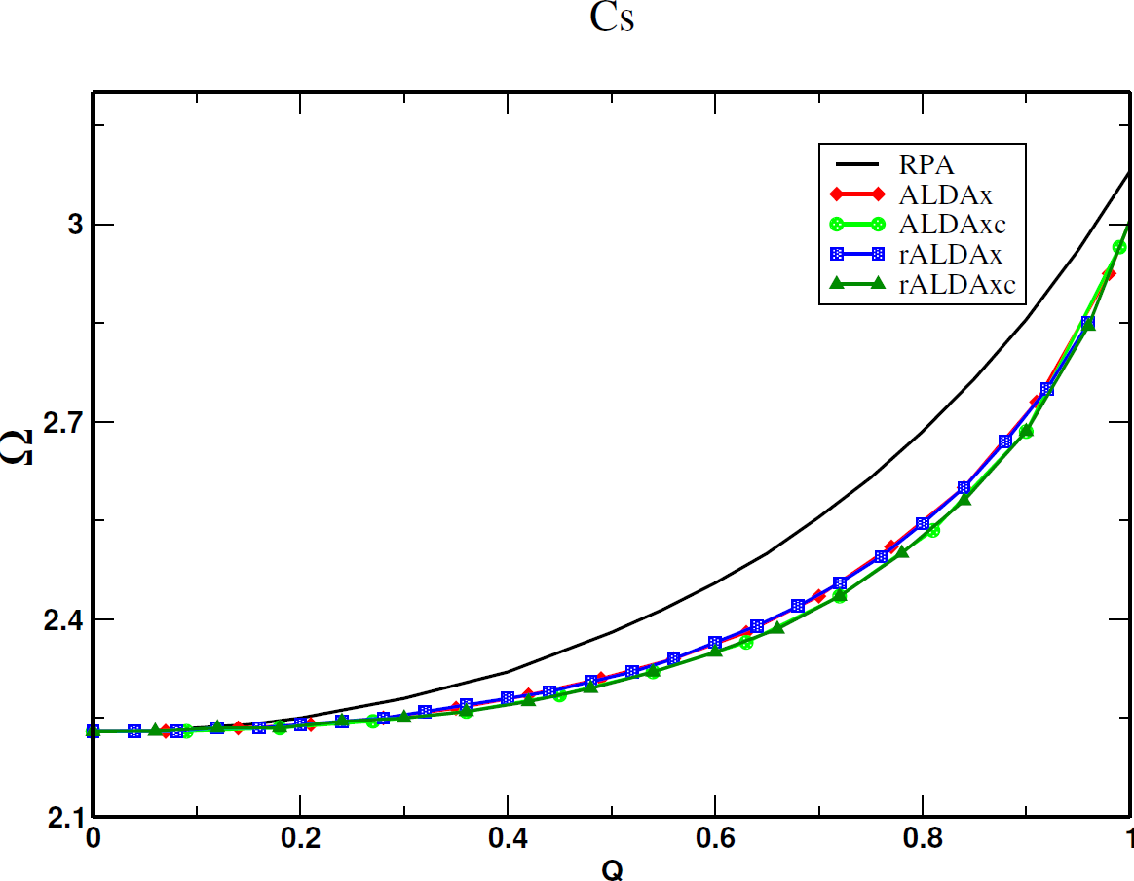
\includegraphics[width=0.45\textwidth]{./media/image3.png}
	\end{subfigure}
~	\begin{subfigure}		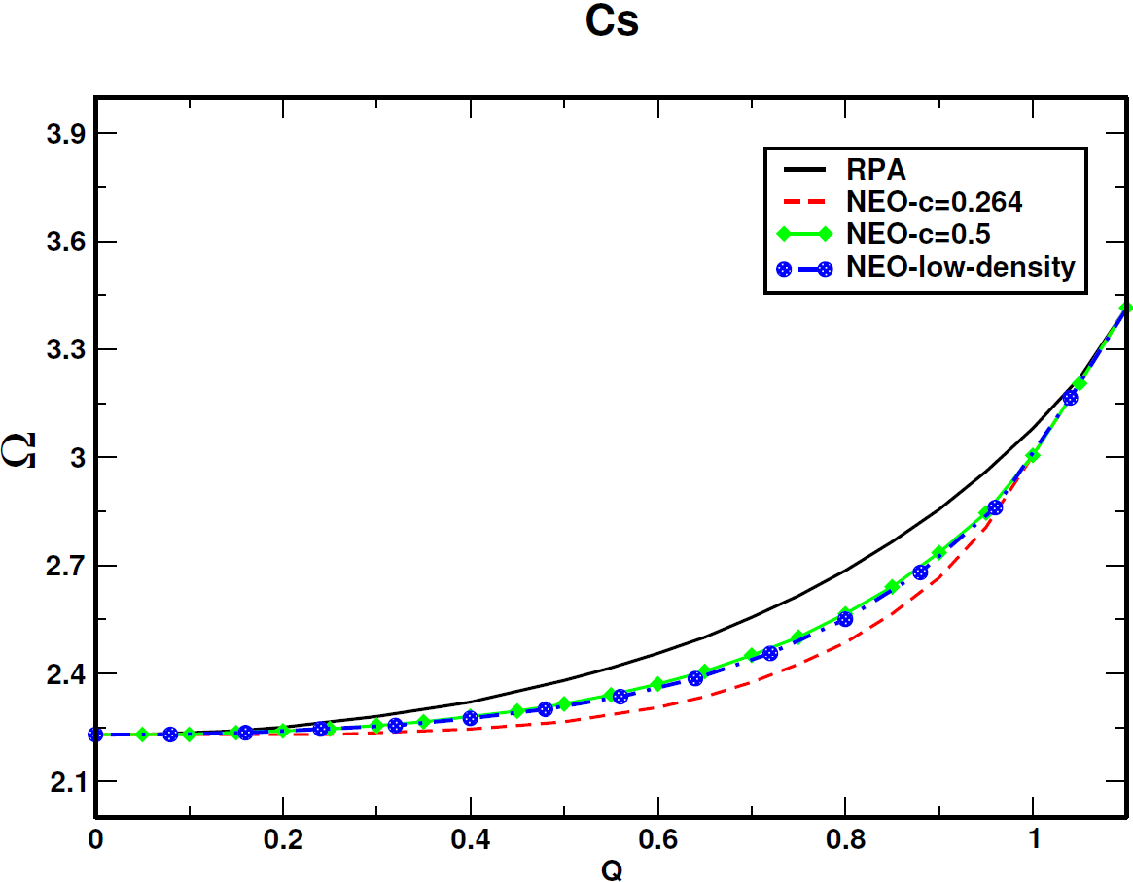
\includegraphics[width=0.45\textwidth]{./media/image12.png}
	\end{subfigure}
~
\end{figure}


%%%%%%%%%%%%%%%%%%%% Figure/Image No: 3 Ends here %%%%%%%%%%%%%%%%%%%%

\setlength{\parskip}{0.0pt}
\par


\vspace{\baselineskip}
\setlength{\parskip}{9.96pt}

\vspace{\baselineskip}
\setlength{\parskip}{0.0pt}
\setlength{\parskip}{9.96pt}
\setlength{\parskip}{0.0pt}
\begin{justify}
\textbf{Fig 3. }The plasmon dispersion for Cs up to the critical wavevector. The left panel shows the dispersion obtained with RPA and beyond-RPA with ALDAx, ALDAxc, rALDAx and rALDAxc approximations. The right panel shows the dispersion from RPA and the three NEO approximations with the c parameters corresponding to different choices.
\end{justify}\par


\vspace{\baselineskip}
\setlength{\parskip}{9.96pt}

\vspace{\baselineskip}
\setlength{\parskip}{0.0pt}
\setlength{\parskip}{9.96pt}
\setlength{\parskip}{0.0pt}
\begin{justify}
To summarize the role of the exact constraints we compare all the exchange and exchange-correlation models described above. We have added NEO c=0.021 to our analysis in Figure 4. Within this version of NEO the  \( \widetilde{c} \)  parameter is $``$reverse-engineered$"$  from Equation (13) of Ref. \textsuperscript{31} to match the density of Cs. This construction loses the exact behavior at  \( q \rightarrow 0. \) 
\end{justify}\par

\begin{justify}
Figure 4 displays the small wavevector behavior of all kernels and with RPA. The exact dispersion relation is known to be quadratic in the wavevector q as E $ \sim $   \( q^{2} \) . Except NEO  \( \widetilde{c}=0.0037, \)  all exchange and exchange-correlation kernels and RPA are properly horizontal at small Q wavevectors and become properly quadratic as Q increase. The horizontal line is a consequence of the exact physical constraints satisfied by these methods. NEO  \( \widetilde{c}=0.0037 \)  is not consistent with the exact constraint of the compressibility sum rule. While NEO  \( \widetilde{c}=0.264 \) \ is based on the exact RPA-like high-density limit, the two unphysical NEO’s deviate from this constraint and pick up a wrong negative quadratic dispersion.  
\end{justify}\par


\vspace{\baselineskip}
\setlength{\parskip}{9.96pt}


%%%%%%%%%%%%%%%%%%%% Figure/Image No: 4 starts here %%%%%%%%%%%%%%%%%%%%

\begin{figure}[H]
	\begin{Center}
		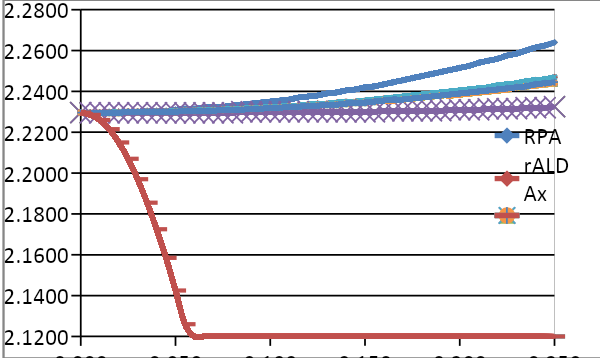
\includegraphics[width=3.55in,height=2.12in]{./media/image7.png}
	\end{Center}
\end{figure}


%%%%%%%%%%%%%%%%%%%% Figure/Image No: 4 Ends here %%%%%%%%%%%%%%%%%%%%

\setlength{\parskip}{0.0pt}
\par


\vspace{\baselineskip}
\setlength{\parskip}{9.96pt}

\vspace{\baselineskip}
\setlength{\parskip}{0.0pt}
\setlength{\parskip}{9.96pt}
\setlength{\parskip}{0.0pt}
\begin{justify}
\textbf{Fig 4}.\  The long wavelength behavior or all approximations considered in this work.
\end{justify}\par


\vspace{\baselineskip}
\setlength{\parskip}{9.96pt}

\vspace{\baselineskip}
\setlength{\parskip}{0.0pt}
\setlength{\parskip}{9.96pt}


%%%%%%%%%%%%%%%%%%%% Figure/Image No: 5 starts here %%%%%%%%%%%%%%%%%%%%

\begin{figure}[H]
	\begin{Center}
		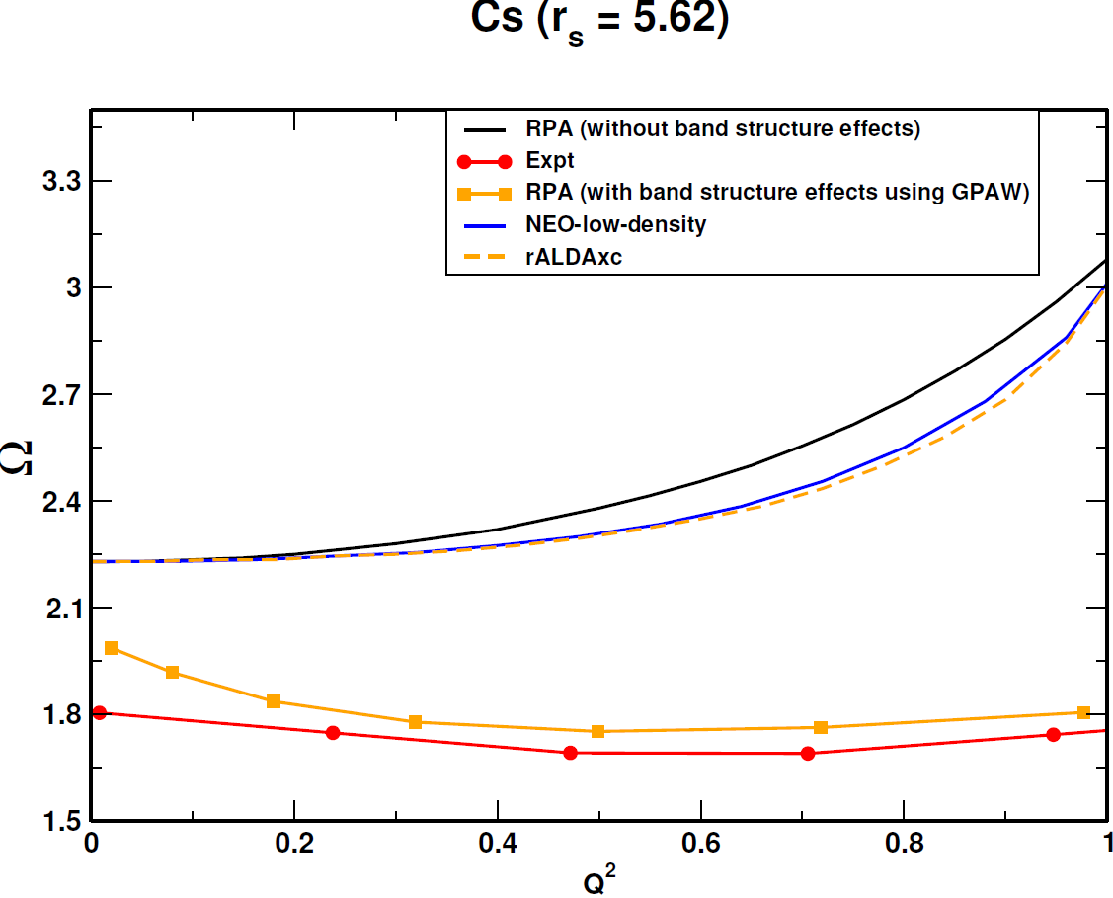
\includegraphics[width=3.24in,height=2.61in]{./media/image1.png}
	\end{Center}
\end{figure}


%%%%%%%%%%%%%%%%%%%% Figure/Image No: 5 Ends here %%%%%%%%%%%%%%%%%%%%

\setlength{\parskip}{0.0pt}
\par


\vspace{\baselineskip}
\setlength{\parskip}{9.96pt}
\setlength{\parskip}{0.0pt}
\begin{justify}
\textbf{Fig 5}.\  
\end{justify}\par


\vspace{\baselineskip}
\setlength{\parskip}{9.96pt}

\vspace{\baselineskip}
\setlength{\parskip}{0.0pt}
\setlength{\parskip}{9.96pt}
\setlength{\parskip}{0.0pt}
\begin{justify}
\textbf{The dynamic structure factor within and beyond-RPA}
\end{justify}\par


\vspace{\baselineskip}
\setlength{\parskip}{9.96pt}
\setlength{\parskip}{0.0pt}
\begin{justify}
The dynamic structure factor \textsuperscript{16} delivers further qualitative and quantitative information about the limitations of our approximations within linear response TDDFT. The dynamic structure factor  \( S \left( q, \omega  \right)  \)  is proportional to  \( Im  \chi  \)  \textsuperscript{34}.  \( Im  \chi  \)  is the loss component of the dynamic density-density response function that designates the dominant plasmon resonance of the spectral function.
\end{justify}\par

\begin{justify}
Using the dynamic structure factor we test our methods and compare the spectral functions to the plasmon dispersion obtained with the same approximations. The structure factor at different q wavevectors defines the dispersion, but showing  \( S \left( q, \omega  \right)  \)  at one particular q only we can gain further insight about the plasmon resonance with various approximations.
\end{justify}\par

\begin{justify}
In Figure 6 we analyze our approximations at three wavevectors:  \( q=0.1k_{F}, \)   \( q=0.5k_{F}, \) \  and  \( q=k_{F}. \)  The latter wavevector is the one at which the plasmons decay into the electron-hole continuum at r\textsubscript{s} = 4.
\end{justify}\par

\begin{justify}
The first figure (a) compares RPA with the default NEO kernel with  \( \widetilde{c}=0.264. \)  The line shapes at  \( q=0.1k_{F} \)  and  \( q=0.5k_{F} \)  are very similar for both methods. At  \( q=k_{F} \)  the line shape of NEO becomes broader than the one of RPA. This finding is to large extent in accord with the recent observation by Lewis and Berkelbach \textsuperscript{35}. However, we have to be careful not to equate our particle-hole (ph) RPA-based methods with EOM-CCSD with ladder diagrams included. Unlike EOM-CCSD, none of the NEO kernels is expected to predict multipair decay channels. If band structure effects are included, no static (ph)RPA-based exchange-correlation kernel can step beyond the ALDA quality dispersion for low-density alkali metals, while an RPA-based method with ladder diagrams may. The plasmon peak is shifted to lower frequencies with the kernel correction compared to RPA.
\end{justify}\par

\begin{justify}
Figure 6.b compares three NEO kernels at r\textsubscript{s} = 4 for the same three wavevectors.
\end{justify}\par


\vspace{\baselineskip}
\setlength{\parskip}{9.96pt}

\vspace{\baselineskip}
\setlength{\parskip}{0.0pt}
\setlength{\parskip}{9.96pt}


%%%%%%%%%%%%%%%%%%%% Figure/Image No: 6 starts here %%%%%%%%%%%%%%%%%%%%


\begin{figure}[H]	\begin{subfigure}		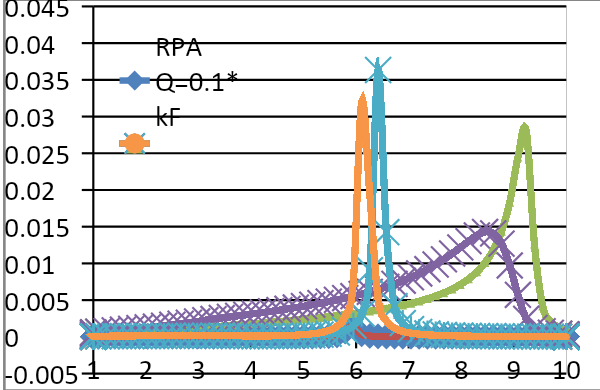
\includegraphics[width=0.45\textwidth]{./media/image11.png}
	\end{subfigure}
~	\begin{subfigure}		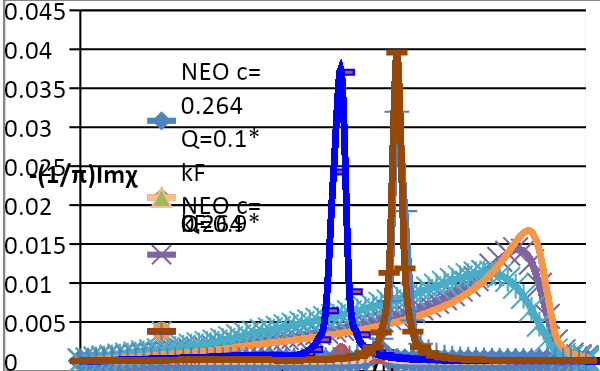
\includegraphics[width=0.45\textwidth]{./media/image10.png}
	\end{subfigure}
~
\end{figure}


%%%%%%%%%%%%%%%%%%%% Figure/Image No: 6 Ends here %%%%%%%%%%%%%%%%%%%%

\setlength{\parskip}{0.0pt}
\par


\vspace{\baselineskip}
\setlength{\parskip}{9.96pt}

\vspace{\baselineskip}
\setlength{\parskip}{0.0pt}
\setlength{\parskip}{9.96pt}


%%%%%%%%%%%%%%%%%%%% Figure/Image No: 7 starts here %%%%%%%%%%%%%%%%%%%%

\begin{figure}[H]
	\begin{Center}
		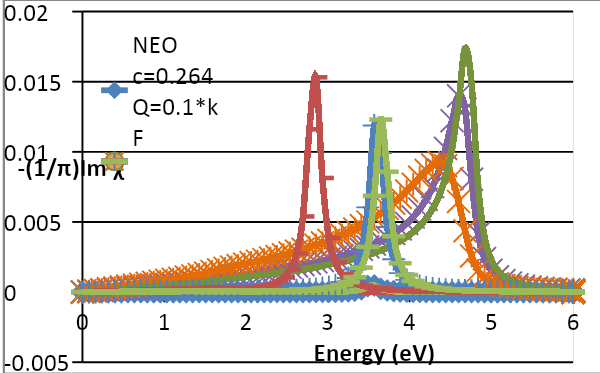
\includegraphics[width=3.27in,height=2.04in]{./media/image4.png}
	\end{Center}
\end{figure}


%%%%%%%%%%%%%%%%%%%% Figure/Image No: 7 Ends here %%%%%%%%%%%%%%%%%%%%

\setlength{\parskip}{0.0pt}
\par


\vspace{\baselineskip}
\setlength{\parskip}{9.96pt}

\vspace{\baselineskip}
\setlength{\parskip}{0.0pt}
\setlength{\parskip}{9.96pt}

\vspace{\baselineskip}
\setlength{\parskip}{0.0pt}
\setlength{\parskip}{9.96pt}
\setlength{\parskip}{0.0pt}
\begin{justify}
\textbf{Fig. 6 }a: the spectral functions for RPA and NEO\textbf{  \( \widetilde{c}=0.264 \) } at r\textsubscript{s }= 4. b: the spectral functions for three NEO kernels at r\textsubscript{s}=4. c: the spectral functions for three NEO kernels at r\textsubscript{s}=5.62 corresponding to Cs.
\end{justify}\par


\vspace{\baselineskip}
\setlength{\parskip}{9.96pt}
\setlength{\parskip}{0.0pt}
\begin{justify}
We have performed another test with the dynamic structure factor. This test is conclusive about the correlation effects in Cs and completes our plasmon dispersion analysis with a justification why a negative dispersion can not exist in Cs.
\end{justify}\par

\begin{justify}
 Exchange-correlation kernels can be applied to improve the ground state correlation energy of RPA through the adiabatic connection fluctuation dissipation theorem. This is the basis of the wavevector decomposition of the ground state exchange-correlation energy as known from Langreth and Perdew \textsuperscript{16}:
\end{justify}\par


\vspace{\baselineskip}
\setlength{\parskip}{9.96pt}
\setlength{\parskip}{0.0pt}
\begin{Center}
\ \ \ \ \ \ \ \ \ \ \ \ \ \ \ \ \ \ \ \ \ \ \ \ \ \ \ \ \ \ \ \ \ \   \( E_{xc}= \int _{}^{}\frac{d^{3}k}{ \left( 2 \pi  \right) ^{3}}\frac{1}{2} \int _{0}^{1}\frac{d \lambda }{ \lambda } \left( \frac{4 \pi  \lambda }{k^{2}} \right) N \left[ S_{ \lambda } \left( k \right) -1 \right] , \) \ \ \ \ \ \ \ \ \ \ \ \ \ \ \ \ \ \ \ \ \ \ \ \ \ \ \ \ \ \ \ \ \ \ \ \ \ \ \ \ \ \ \ \ \ \ \ \ \ \ \ \ \ \ \ \ \  (9)
\end{Center}\par


\vspace{\baselineskip}
\setlength{\parskip}{9.96pt}
\setlength{\parskip}{0.0pt}
\begin{justify}
where $ \lambda $  is the coupling constant along the adiabatic connection path and  \( S_{ \lambda } \left( k \right)  \)  is the frequency-integrated Fourier transform of the static structure factor in the position space. According to the expression given by (9), the exchange-correlation energy is proportional to the dynamic structure factor.
\end{justify}\par

\begin{justify}
Figure 7 shows the wavevector decomposition of of all exchange and exchange-correlation kernels within Equation (9) for the correlation-only energy. We plot the correlation energy for r\textsubscript{s} = 5.62. 
\end{justify}\par

\begin{justify}
The\ physical basis of our analysis is the exact exchange-correlation kernel   \( f_{xc} \left( q, \omega  \right)  \)  of the uniform electron gas. For the correlation energy the static version of this quantity is  \( f_{xc} \left( q,0 \right)  \)  can be applied \textsuperscript{22}. The ALDA exchange-correlation kernel  \( f_{xc}^{ALDA} \left( q,0 \right)  \)  is approaching the exact kernel for the uniform electron gas at  \( q \rightarrow 0. \) \  Note that the frequency dependence at least qualitatively can be also ignored for  \(  \omega  \approx  \omega _{p} \)  \textsuperscript{36, 37}.\  By the long wavelength behavior of ALDA:
\end{justify}\par


\vspace{\baselineskip}
\setlength{\parskip}{9.96pt}
\setlength{\parskip}{0.0pt}
\begin{Center}
\ \ \ \ \ \ \ \ \ \ \ \ \ \ \ \ \ \ \ \ \ \ \ \ \ \ \ \ \ \ \ \ \ \ \ \ \ \ \ \ \   \( f_{xc} \left( q,0 \right) =f_{xc}^{ALDA} \left( q,0 \right) ~, \) \ \ \ \ \ \ \ \ \ \ \ \ \ \ \ \ \ \ \ \ \ \ \ \ \ \ \ \ \ \ \ \ \ \ \ \ \ \ \ \ \ \ \ \ \ \ \ \ \ \ \ \ \ \ \ \ \ \ \ \ \  (10)
\end{Center}\par


\vspace{\baselineskip}
\setlength{\parskip}{9.96pt}
\setlength{\parskip}{0.0pt}
therefore:\par


\vspace{\baselineskip}
\setlength{\parskip}{9.96pt}
\setlength{\parskip}{0.0pt}
\begin{Center}
\ \ \ \ \ \ \ \ \ \ \ \ \ \ \ \ \ \ \ \ \ \ \ \ \ \ \ \ \ \ \ \ \ \ \ \ \ \ \ \ \ \ \ \ \ \ \   \( f_{xc}^{ALDA} \left( q,0 \right) <f_{xc} \left( q,0 \right) <0. \) \ \ \ \ \ \ \ \ \ \ \ \ \ \ \ \ \ \ \ \ \ \ \ \ \ \ \ \ \ \ \ \ \ \ \ \ \ \ \ \ \ \ \ \ \ \ \ \ \ \ \ \ \ \ \ \ \ \  (11)
\end{Center}\par


\vspace{\baselineskip}
\setlength{\parskip}{9.96pt}
\setlength{\parskip}{0.0pt}
\begin{justify}
The\ ALDA approximation becomes a lower bound to the static exact exchange-correlation kernel for the correlation energy of the uniform electron gas. Figure 7 visualizes the relation between ALDAc, RPA and some other exchange-correlation kernels.  The ALDAc is shown in the left panel of Figure 7. The ALDAc is very accurate for small wavevectors but starts deviate from RPA at  \( Q \approx 0.25. \)  At \(  k=2k_{F} \)  the ALDAc becomes a strong overestimation of the RPA correlation energy.
\end{justify}\par

\begin{justify}
All other beyond-RPA kernels make the exchange-correlation energy of RPA less negative for any density including r\textsubscript{s} = 5.62. The correlation energies from NEO  \( \widetilde{c}=0.264 \)  and NEO  \( kernel fitted against the compressibility sum-rule \)  are close to each other but the unphysical NEO  \( \widetilde{c}=0.0037 \)  adds a much larger correction to the RPA correlation energy. Although NEO  \( \widetilde{c}=0.0037 \)  appears to be a better correction to the RPA ground state energy; this correction may not be transferable to inhomogeneous systems as indicated in Ref. \textsuperscript{24}. Interestingly, the same exact physical constraints control the plasmon dispersion and damping as the one the ground state correlation energy.
\end{justify}\par

\begin{justify}
The constraints by Equations (10) and (11) determine the correlation energy of all other exchange and exchange-correlation kernels. The dynamic structure factor becomes a link that couples the physics in the correlation energy and plasmon dispersion. Through the correlation energy of ALDA no uniform-electron gas-based kernel can be more negative than ALDAc in the correlation energy and no more negative in the plasmon dispersion. The NEO  \( \widetilde{c}=0.264 \)  kernel is uniform electron gas-based only through its energy optimization to the high-density limit.
\end{justify}\par


\vspace{\baselineskip}
\setlength{\parskip}{9.96pt}

\vspace{\baselineskip}
\setlength{\parskip}{0.0pt}
\setlength{\parskip}{9.96pt}

\vspace{\baselineskip}
\setlength{\parskip}{0.0pt}
\setlength{\parskip}{9.96pt}


%%%%%%%%%%%%%%%%%%%% Figure/Image No: 8 starts here %%%%%%%%%%%%%%%%%%%%


\begin{figure}[H]	\begin{subfigure}		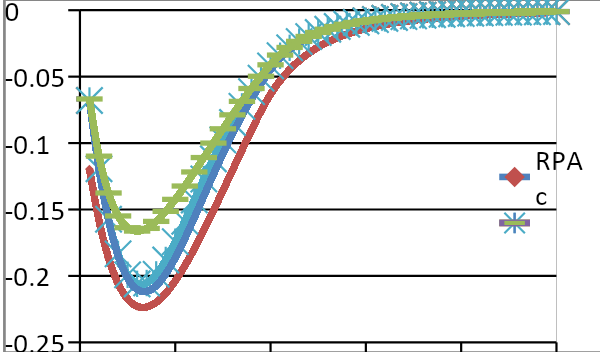
\includegraphics[width=0.45\textwidth]{./media/image8.png}
	\end{subfigure}
~	\begin{subfigure}		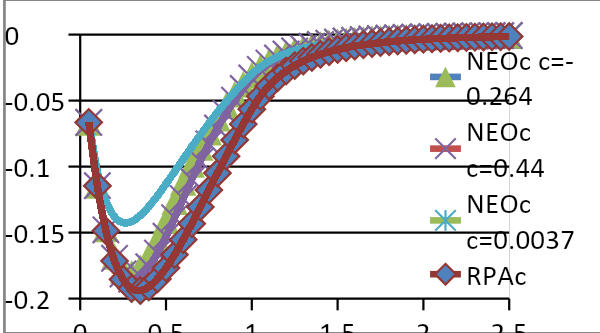
\includegraphics[width=0.45\textwidth]{./media/image9.png}
	\end{subfigure}
~
\end{figure}


%%%%%%%%%%%%%%%%%%%% Figure/Image No: 8 Ends here %%%%%%%%%%%%%%%%%%%%

\setlength{\parskip}{0.0pt}
\begin{justify}
 
\end{justify}\par


\vspace{\baselineskip}
\setlength{\parskip}{9.96pt}

\vspace{\baselineskip}
\setlength{\parskip}{0.0pt}
\setlength{\parskip}{9.96pt}
\setlength{\parskip}{0.0pt}
\begin{justify}
\textbf{Fig. 7. }Wavevector analysis of the ground state correlation-only energy from the dynamic structure factor for reduced wavevector  \( Q=\frac{k}{2k_{F}}. \)  The left figure shows the correlation-only energy for RPA, ALDA and NEO with the three choices for  \( \widetilde{c}, \)  for r\textsubscript{s}=4. The right figure shows the same for r\textsubscript{s}=5.62 corresponding to Cs.
\end{justify}\par


\vspace{\baselineskip}
\setlength{\parskip}{9.96pt}

\vspace{\baselineskip}
\setlength{\parskip}{0.0pt}
\setlength{\parskip}{9.96pt}

\vspace{\baselineskip}
\setlength{\parskip}{0.0pt}
\setlength{\parskip}{9.96pt}
\setlength{\parskip}{0.0pt}
\begin{justify}
\textbf{Conclusion }
\end{justify}\par


\vspace{\baselineskip}
\setlength{\parskip}{9.96pt}
\setlength{\parskip}{0.0pt}
\begin{justify}
We have presented various model exchange-correlation kernels beyond-RPA for the plasmon dispersion within the jellium model for alkali metals. Most of these approximations are based on the uniform electron gas paradigm. We show that the plasmon damping mechanism is strictly controlled by exact constraints. Furthermore we also demonstrate that electronic excitations such as plasmons require different physics built in the approximations. Additional physics such as nonlocality in space imposed to ground state can be meaningless for plasmon excitations. In change, physical constraints as the compressibility sum rule determine the plasmon decay with exchange-correlation kernels. Clearly any of our methods based on particle-hole RPA is not able to predict the experimentally observed negative plasmon dispersion for the heavy alkali metal Cs. The current exchange-correlation kernels do not have an explicit density dependence that could have a larger impact. For all the model exchange-correlation kernels the ALDAxc is a lower bound. The ALDAxc is accurate for  \( \frac{q}{k_{F}}<1, \)  the range of  \( q \)  that determines the plasmon dispersion, even though the ALDAxc kernel fails badly for  \( \frac{q}{k_{F}} \gg 1. \) \  Beside correlation, frequency dependence can influence the plasmon damping, however, this remains to be investigated in an upcoming work.
\end{justify}\par


\vspace{\baselineskip}
\setlength{\parskip}{9.96pt}

\vspace{\baselineskip}
\setlength{\parskip}{0.0pt}
\setlength{\parskip}{9.96pt}
\setlength{\parskip}{0.0pt}
\begin{justify}
\textbf{Acknowledgment:} The research of N.K.N., S.R. and A.R. was supported by the National Science Foundation under Grant {\fontsize{10pt}{12.0pt}\selectfont No.DMR-1553022\par}.
\end{justify}\par


\vspace{\baselineskip}
\setlength{\parskip}{9.96pt}

\vspace{\baselineskip}
\setlength{\parskip}{0.0pt}
\setlength{\parskip}{9.96pt}

\vspace{\baselineskip}
\setlength{\parskip}{0.0pt}
\setlength{\parskip}{9.96pt}

\vspace{\baselineskip}
\setlength{\parskip}{0.0pt}
\setlength{\parskip}{9.96pt}
\setlength{\parskip}{0.0pt}
\begin{enumerate}
	\item G. Onida, L. Reining, and A. Rubio, Rev. Mod. Phys, \textbf{74}, 601 (2002)\par

	\item H. Reather, Excitations of Plasmons and Interband Transitions by Electrons (Springer-Verlag, Berlin, 1980)\par

	\item W. Schülke, J.R. Schimts, H. Schulte-Schrepping, and A. Kaprolat, Phys. Rev. B \textbf{52}, 11721 (1995) \par

	\item E. Runge and E. K. U. Gross, Phys. Rev. Lett. \textbf{52},\ 997  (1984)\par

	\item D. Pines, Elementary Excitations in Solids (Benjamin, New York, 1964)\par

	\item M. Petersilka, U.J. Gossmann, and E.K.U. Gross, Phys. Rev. Lett. \textbf{52},\ 997  (1984)\par

	\item A. vom Felde, J. Sprösser-Prou, and J. Fink, Phys. Rev. B \textbf{40}, 10181 (1989)\par

	\item D. Pines and P. Nozières, The Theory of Quantum Liquids, (Benjamin, New York, 1966) Vol. 1.\par

	\item F. Aryasetiawan, K. Karlsson, Phys. Rev. Lett. \textbf{73}, 1679 (1994)\par

	\item W. Ku and A. Eguiluz, Phys. Rev. Lett. \textbf{82}, 2350 (1999)\par

	\item M. Taut, J. Phys. Condens. Matter, \textbf{4}, 9595 (1992)\par

	\item M. Taut and K. Sturm, Solid State Comm. 82, 295 (1992)\par

	\item D. Bohm and D. Pines, Phys. Rev. \textbf{92}, 609 (1953)\par

	\item D.C. Langreth and J.P. Perdew, Solid State Commun. \textbf{17,} 1425 (1975)\textbf{\  }\par

	\item D.C. Langreth and J. P. Perdew, Phys. Rev. B \textbf{15}, 2884 (1977)\par

	\item K. Tatarczyk, A. Achindmayr, and M. Scheffler, Phys Rev. B, \textbf{63}, 235106 (2001)\par

	\item J. Sun et al., Nature Chem., \textbf{8}, 831 (2016)\par

	\item \textcolor[HTML]{222222}{J. P. Perdew, A. Ruzsinszky, J. Tao, V. N. Staroverov, G. E. Scuseria, G. I. Csonka, J. Chem. Phys. \textbf{123}, 062201 (2005)}\par

	\item \textcolor[HTML]{222222}{J. Lindhard, Dan. Mat. Fys. Medd. \textbf{28}, 8 (1954)}\par

	\item A. Zangwill and P. Soven, Phys. Rev. A \textbf{21},\ 1561  (1980)\par

	\item M.\ Lein, E.K.U. Gross, J.P. Perdew, Phys. Rev. B,  \textbf{61}, 13431 (2000)\par

	\item T. Olsen, and K.S. Thygesen, \textbf{86},\ 081103(R)  (2012)\par

\setlength{\parskip}{11.28pt}
	\item J. E. Bates, S. Laricchia, and A. Ruzsinszky, Phys. Rev. B \textbf{93}, 045119 (2016)\par

	\item C. F. von Weizsäcker, Z. Phys. \textbf{96}, 431 (1935)\par

\setlength{\parskip}{0.0pt}
	\item U. von Barth and L. Hedin, J. Phys. C \textbf{5}, 1629 (1972), and references therein.\par

	\item L. A. Constantin and J. M. Pitarke, Phys. Rev. B, \textbf{75},{\fontsize{9pt}{10.8pt}\selectfont  \par}245127 (2007)\par

	\item S. Ichimaru, Rev. Mod. Phys. \textbf{54}, 1017 (1982)\par

	\item K. S. Singwi, M. P. Tosi, R. H. Land, and A. Sjölander, Phys. Rev. \textbf{176}, 589 (1968)\par

	\item A. A. Quong, A. G. Eguiluz, Phys. Rev. Lett. \textbf{70}, 3955 (1993)\par

\setlength{\parskip}{11.28pt}
	\item A. Ruzsinszky, L.A. Constantin and J.M. Pitarke, Phys. Rev. B \textbf{94}, 165155 (2016)\par

\setlength{\parskip}{0.0pt}
	\item E. Petri and A. Otto, Phys. Rev. Lett. \textbf{34}, 1283 (1975)\par

	\item A. Fleszar, R. Stumpf, A. G. Eguiluz, Phys. Rev. B, \textbf{55}, 2068 (1997)\par

	\item E. Jensen, and W. Plummer, Phys. Rev. Lett. \textbf{55}, 1912 (1985); P.H. Citrin et al, \textit{ibid}. \textbf{61}, 1021 (1988); B. S. Itchkawitz et al., \textit{ibid}. \textbf{68}, 2488 (1993)\par

	\item A. M. Lewis, T. C. Berkelbach, Phys. Rev. Lett. \textbf{122}, \textcolor[HTML]{222222}{226402 (2019)}\par

	\item N. Iwamoto, E. K. U. Gross, Phys. Rev. B, \textbf{35}, 3003 (1987)\par

	\item E. K. U. Gross and W. Kohn, Phys. Rev. Lett. \textbf{55}, 2850 (1985)\par


\vspace{\baselineskip}
\setlength{\parskip}{9.96pt}

\vspace{\baselineskip}
\setlength{\parskip}{0.0pt}
\setlength{\parskip}{9.96pt}
\setlength{\parskip}{0.0pt}
\begin{enumerate}
	\item D.C. Langreth and J. P. Perdew, Phys. Rev. B \textbf{21}, 5469 (1980)\par

	\item P. Nozières and D. Pines, Phys. Rev. 113, 1254 (1969)\par

	\item D.F. DuBois and M.G. Kivelson, Phys. Rev. 186, 409 (1969)
\end{enumerate}\par

C.F. Richardson and N.W. Ashcroft, Phys. Rev. B \textbf{50}, 8170 (1994)\par


\vspace{\baselineskip}
\setlength{\parskip}{9.96pt}

\vspace{\baselineskip}
\setlength{\parskip}{0.0pt}
\setlength{\parskip}{9.96pt}

\vspace{\baselineskip}
\setlength{\parskip}{0.0pt}
\setlength{\parskip}{9.96pt}

\end{enumerate}
\printbibliography
\end{document}